%%==================================================
%% demo.tex for BIT Thesis
%% modified by yang yating
%% version: 1.0
%% last update: Sep. 1st, 2017
%%==================================================

% 默认单面打印 oneside 、硕士论文模板 master

\documentclass[oneside, master,normal]{BIT-thesis-grd-jdh}
%\usepackage{mathptmx}
% \usepackage[justification=centering]{caption}
% 打印选项: 双面打印 oneside;单面打印 twoside
% 模板选项: 硕士论文 master; 博士论文 doctor
\usepackage{listings} 
\begin{document}

%%%%%%%%%%%%%%%%%%%%%%%%%%%%%%
%% 封面
%%%%%%%%%%%%%%%%%%%%%%%%%%%%%%

% 中文封面内容(关注内容而不是表现形式)
% \classification{TN914.3}
% \UDC{540}

\title{LaTeX论文写作填坑/拓展指南}
\vtitle{LaTeX论文写作填坑/拓展指南}
\author{JDH}

\defenddate{2019年5月}

% 封面绘制
\maketitle

%%%%%%%%%%%%%%%%%%%%%%%%%%%%%%
%% 前置部分
%%%%%%%%%%%%%%%%%%%%%%%%%%%%%%
\frontmatter
\allowdisplaybreaks

% 加入目录
\tableofcontents

%%%%%%%%%%%%%%%%%%%%%%%%%%%%%%
%% 正主体部分
%%%%%%%%%%%%%%%%%%%%%%%%%%%%%%
\mainmatter

%% 各章正文内容
%\include{chapters/WritingReference}
%%==================================================
%% abstract.tex for BIT Master Thesis
%% Edited by Jian dahao
%% version: 1.0
%% last update: May 10th, 2019
%%==================================================
\chapter{内容不多但一定要看的前言}
\noindent{本文档内容主要包括:}
\begin{enumerate}
\item 模板BIT-thesis-LaTeX简介
\item 使用LaTeX撰写论文过程中遇到的一些坑,以及对应的解决方法记录。
\end{enumerate}
模板BIT-thesis-LaTeX仅仅是在官方模板(地址:\url{https://github.com/BIT-thesis/LaTeX-template})基础上进行更改,其使用方法与官方模板基本一致,所以务必先\textbf{重点参考官方模板中的BIT-Thesis使用指南手册v1.1说明文档},当碰到坑的时候再来该文档碰碰运气,万一这些坑该文档正好给填了呢。。。。该文档结合模板BIT-thesis-LaTeX讲解(项目地址:\url{https://github.com/jiandahao/BIT-thesis-LaTex})。
\\
\\
\begin{center}
{{\fbox{\fbox{\zihao{1}该文档仅供参考                                \zihao{5}<Copyright 2019 by JDH>}}}}
\end{center}
%%==================================================
%% abstract.tex for BIT Master Thesis
%% Edited by Jian dahao
%% version: 1.0
%% last update: May 10th, 2019
%%==================================================
\chapter{模板入门}
重点查看官方模板中的BIT-Thesis使用指南v1.1手册。需要另外说明的是,为了更好的进行文章结构的管理,在章节文件夹中添加了chapter1文件夹用于演示对每一章节文件的组织。此外,新增了配置文件BIT-thesis-grd-jdh.cls,该配置控制文件是基于官方提供的BIT-thesis-grd.cls进行修改,具体区别参见第\ref{section:与官方模板的区别}一节。
\section{模板结构初识}
\begin{lstlisting}[language={tex}, caption={模板文件布局}]
demo.tex      							主控文件
demo.pdf   								生成的pdf文件
BIT-thesis-grd.cls 						官方提供的格式控制文件
BIT-thesis-grd-jdh.cls  				新增的格式控制文件,基于BIT-thesis-grd.cls修
										改,模板默认使用该控制文件
GBT7714-2005NLang  						参考文献格式控制文件<写论文过程中基本不需要修
										改,知道是什么就好了>
chapters 								章节文件夹
		abstract.tex 					摘要
		chapter1 						第一章文件夹
			chapter1.tex 				第一章内容主文件
				chapter1_1.tex 			第一章第一节
				chapter1_2.tex 			第一章第二节
			figures 					第一章图片存储文件夹
		conclusion.tex 					总结
		pub.tex 						攻读学位期间发表论文与研究成果清单
		app1.tex						附录A <无硬性要求,可不加>
		thanks.tex 						致谢
		resume.tex 						个人简历
reference								参考文献管理文件夹
		references.bib 					Bibtex文件,记录参考文献条目
BIT-thesis-run.bat 						Windows 编译脚本
BIT-thesis-run.sh 						Linux 编译脚本
\end{lstlisting}
\section{如何创建章节标题}
\begin{lstlisting}[language={tex}, caption={章节创建命令}]
创建新的章节						\chapter{新章节标题}
创建一级标题						\section{一级标题}
创建二级标题						\subsection{二级标题}
创建三级标题						\subsubsection{三级标题} ,模板中三级标题在正
									文能正常显示,但不会在目录中显示
\end{lstlisting}
具体使用参见模板工程。如果正文中需要对章节进行引用,则可以在章节标题之后添加$\backslash$label
\begin{lstlisting}[language={tex}, caption={添加标签}]
\chapter{新章节标题}\label{chapter:这是一章}
\section{一级标题}\label{chapter:这是一节}

在文中的引用形式为\ref{chapter:这是一章}
\end{lstlisting}
\section{章节结构管理}
由于毕业论文篇幅较大,如果统统只写在一个文件里将非常不便于管理。可将各章节各小节分别写在独立的tex文件里,并且将图片、表格等也用文件夹进行管理。

在主控文件中通过$\backslash$include命令插入文件内容,在其他文件中应使用$\backslash$input命令完文件内容插入。具体请参考模板进行举一反三。
\begin{lstlisting}[language={tex}, caption={如何包含文件}]
demo.tex中: %%==================================================
%% chapter01.tex for BIT Master Thesis
%% modified by yang yating
%% version: 0.1
%% last update: Dec 25th, 2016
%%==================================================
\chapter{绪论}
\label{chap:intro}
%在下方加入各小节内容
\section{本论文研究的目的和意义}

近年来,随着人们生活水平的不断提高,人们越来越注重周围环境对身体健康的影响。作为服装是人们时时刻刻最贴近的环境,尤其是内衣,对人体健康有很大的影响。由于合时刻刻最贴近的环境,尤其是内衣,对人体健康有很大的影响。由于合成纤维的衣着舒适性、手感性,天然纤维的发展又成为人们关注的一大热点。

……\upcite{Takahashi1996Structure,Xia2002Analysis,Jiang1989,Mao2000Motion,Feng1998}
\section{国内外研究现状及发展趋势}
%\label{sec:***} 可标注label

\subsection{形状记忆聚氨酯的形状记忆机理}
%\label{sec:features}

形状记忆聚合物(SMP)是继形状记忆合金后在80年代发展起来的一种新型形状记忆材料\cite{Jiang2005Size}。形状记忆高分子材料在常温范围内具有塑料的性质,即刚性、形状稳定恢复性;同时在一定温度下(所谓记忆温度下)具有橡胶的特性,主要表现为材料的可变形性和形变恢复性。即“记忆初始态-固定变形-恢复起始态”的循环。

固定相只有物理交联结构的聚氨酯称为热塑性SMPU,而有化学交联结构称为热固性SMPU。热塑性和热固性形状记忆聚氨酯的形状记忆原理示意图如图\ref{fig:diagram}所示

\begin{figure}
 \centering
 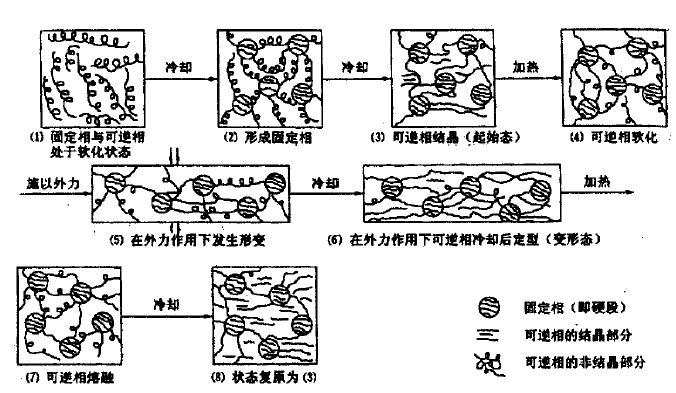
\includegraphics[width=0.75\textwidth]{chapters/chapter1/figures/figure1}
 \caption{热塑性形状记忆聚氨酯的形状记忆机理示意图}\label{fig:diagram}
\end{figure}


\subsection{形状记忆聚氨酯的研究进展}
%\label{sec:requirements}
首例SMPU是日本Mitsubishi公司开发成功的……。

\subsection{水系聚氨酯及聚氨酯整理剂}

水系聚氨酯的形态对其流动性,成膜性及加工织物的性能有重要影响,一般分为三种类型\cite{Jiang2005Size} ,如表 \ref{tab:category}所示。

\begin{table}
  \centering
  \caption{水系聚氨酯分类} \label{tab:category}
  \begin{tabular*}{0.9\textwidth}{@{\extracolsep{\fill}}cccc}
  \toprule
    类别			&水溶型		&胶体分散型		&乳液型 \\
  \midrule
    状态			&溶解$\sim$胶束	&分散		&白浊 \\
    外观			&水溶型		&胶体分散型		&乳液型 \\
    粒径$/\mu m$	&$<0.001$		&$0.001-0.1$		&$>0.1$ \\
    重均分子量	&$1000\sim 10000$	&数千$\sim 20万$ &$>5000$ \\
  \bottomrule
  \end{tabular*}
\end{table}

由于它们对纤维织物的浸透性和亲和性不同,因此在纺织品染整加工中的用途也有差别,其中以水溶型和乳液型产品较为常用。另外,水系聚氨酯又有反应性和非反应性之分。虽然它们的共同特点是分子结构中不含异氰酸酯基,但前者是用封闭剂将异氰酸酯基暂时封闭,在纺织品整理时复出。相互交联反应形成三维网状结构而固着在织物表面。
……



其他非顶层文件:\section{本论文研究的目的和意义}

近年来,随着人们生活水平的不断提高,人们越来越注重周围环境对身体健康的影响。作为服装是人们时时刻刻最贴近的环境,尤其是内衣,对人体健康有很大的影响。由于合时刻刻最贴近的环境,尤其是内衣,对人体健康有很大的影响。由于合成纤维的衣着舒适性、手感性,天然纤维的发展又成为人们关注的一大热点。

……\upcite{Takahashi1996Structure,Xia2002Analysis,Jiang1989,Mao2000Motion,Feng1998}
\end{lstlisting}

\section{与官方模板的区别}
\label{section:与官方模板的区别}
该模板基于官方v1.5版本修改,主要功能区别如下
\begin{enumerate}
\item 新增普通模式(normal)、自查重模式(selfSimilarCheck)和盲审模式(blindCheck)。提交学校的查重文件可以直接使用normal模式结果
;自查重模式主要用于关闭图片、公式等内容的显示,以减少文章字符数和降低PDF转word过程中出现的乱码,节省查重费用支出。应结合$\backslash$insertContents等系列命令使用。对于土豪此选项没有任何卵用。。。。。;盲审模式主要根据盲审文件格式要求,隐去了作者、导师、致谢等信息,更改发表论文的格式
\item 增加$\backslash$makeVerticalenWords命令,修改英文单词树立排放时的显示效果。
\item 增加书脊中作者姓名显示。
\item 增加对mathptmx包的引用,修改公式字体为New Time Roman。
\item{新增$\backslash$pubitem命令,用于显示学术成果。在盲审模式下该命令将会隐去作者信息。}
\item{新增$\backslash$sayThanks命令,用于致谢。在盲审模式下该命令指定的致谢内容将不被显示。}
\item{新增$\backslash$insertContents、$\backslash$insertFigure、$\backslash$insertTable、$\backslash$insertEquation系列指令,该指令用于自查重模式下选择性指定不显示的内容。}
\item{新增$\backslash$ncite、$\backslash$nupcite、$\backslash$nref命令,自查重模式下将不显示}
\item{修复了官方v1.5版本中文献引用标注显示的字号和颜色。}
\item{目录中章节标题取消加粗显示}
\item{打印中文信息的命令更改为$\backslash$makeChineseInfo}
\item{修改英文信息中下划线的长度。}
\end{enumerate}
%%==================================================
%% abstract.tex for BIT Master Thesis
%% Edited by Jian dahao
%% version: 1.0
%% last update: May 10th, 2019
%%==================================================
\chapter{数学公式使用}
数学公式的使用可先参考官方模板中的BIT-Thesis使用指南。
\section{公式编辑}
LaTeX公式是通过代码的形式进行编辑,运算符号、特殊字母等数学符号对应的命令可参考链接\url{http://www.mohu.org/info/symbols/symbols.htm}。不会写代码或者不想敲代码怎么办,可以通过MathType、LaTeX公式在线编辑工具等进行编辑,然后导出tex代码。
\subsection{用MathType编辑}
首先你需要一个已经破解的MathType工具。打开MathType后在设置剪切复制选项。
\begin{figure}[h]
\centering
 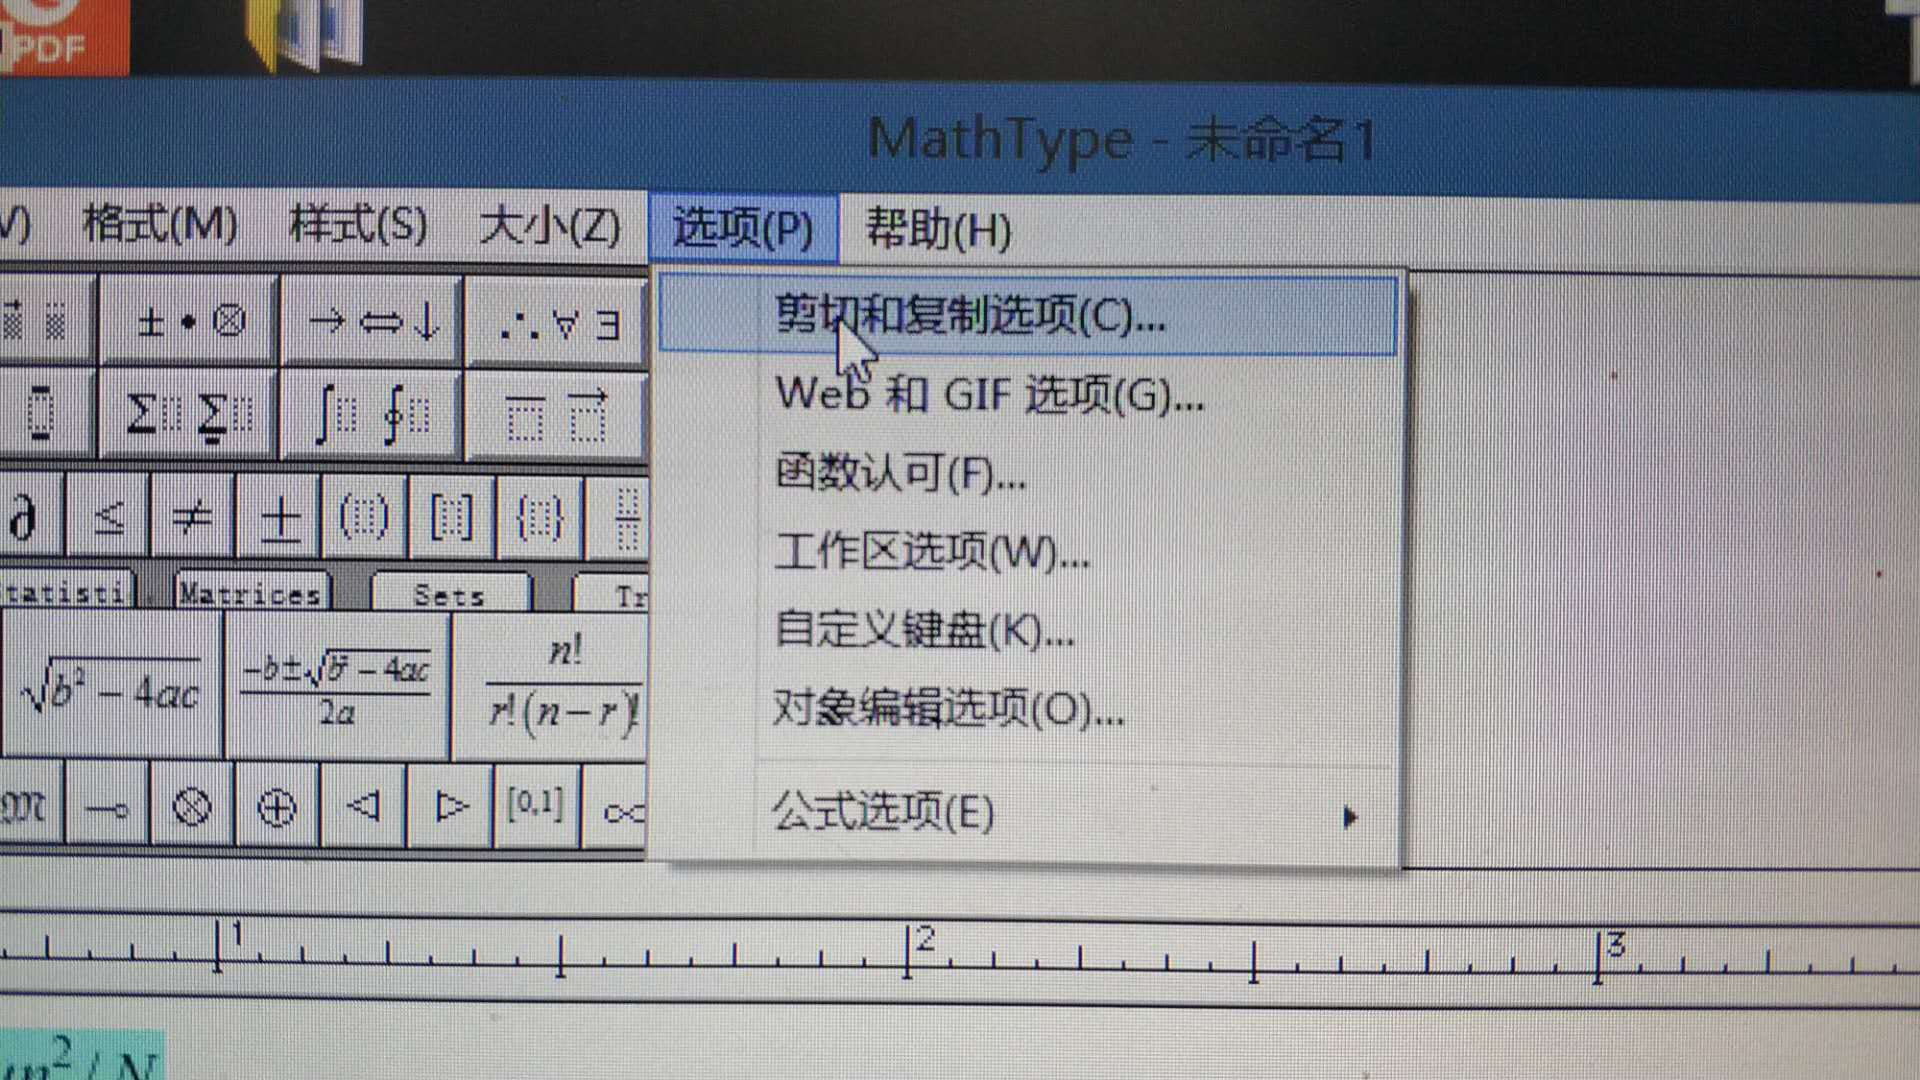
\includegraphics[width=0.75\textwidth]{HelperSection/figures/mathtype_copy_type.jpg}
\end{figure}
然后在\textbf{转换其他文字}中选择\textbf{Plain Tex}或者\textbf{LaTeX 2.09 and later},诸如此类即可。

用MathType编辑好公式后,只需全选复制或剪切就能获得公式代码,例如公式
\begin{equation}
A(n) = e^{4j\pi \mu n^2/N} \notag
\end{equation}
对应的导出结果为:\\
% \begin{lstlisting}[language={tex}, caption={插入公式基本操作}]
Plain Tex:\textbf{\$\$}A(n)\{\rm\{ = \}\}\{e\^\ \{4j$\backslash$pi $\backslash$mu \{n\^\ 2\}/N\}\}\textbf{\$\$} \\
Latex 2.09 and later: $\backslash$[A(n)\{$\backslash$rm\{ = \}\}\{e\^\ \{4j$\backslash$pi $\backslash$mu \{n\^\ 2\}/N\}\}$\backslash$]

需要注意的是,导出的tex代码中需要删除对应的前缀和后缀:对于\textbf{Plain Tex}为\$\$;对\textbf{Latex 2.09 and later}为$\backslash$[ $\quad$ $\backslash$]。

\begin{figure}[h]
\centering
 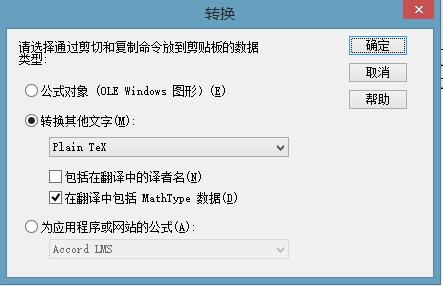
\includegraphics[width=0.75\textwidth]{HelperSection/figures/copy_type.jpg}
\end{figure}
\subsection{用在线工具编辑}
推荐两个网站

\url{http://latex.codecogs.com/eqneditor/editor.php}

\url{https://www.codecogs.com/latex/eqneditor.php}

个人还是比较推荐学一下基本的tex公式语法(边用边学就好),这样写起来会快很多。

\section{怎么插入公式}
% \subsection{段落间插入公式}
对于插入到段落之间的且需要编号公式其定义的内容需要被包含在$\backslash$begin\{equation\}$\backslash$end \{equation\} 之间,基本使用方法如下:
\begin{lstlisting}[language={tex}, caption={插入公式基本操作}]
\begin{equation}
A(n) = e^{4j\pi \mu n^2/N}
\end{equation}
\end{lstlisting}
插入效果为:
\begin{equation}
A(n) = e^{4j\pi \mu n^2/N}
\end{equation}
% \subsection{文本中插入公式}
而对于插入到文本中间的公式只需将公式内容用一对\$\$包起来即可,例如:
这是一段文本这里要插入的公式用法为\$2\^\ \{n\}\$,对应的效果为$2^{n}$。
\section{公式换行与跨页}
由于经常会遇到插入的数学公式巨长,无法在一行上正常显示,或者为了排版美观而需要进行强制换行,常用方法如下。
\subsection{公式换行之基本操作}
\label{sec:公式换行之基本操作}
\vspace{-1cm}
\begin{lstlisting}[language={tex}, caption={结合split和equation环境插入公式}]
\begin{equation}
\begin{split}
A(n) &= e^{4j\pi \mu n^2/N} \\
&= e^{4j\pi \mu n^2/N}
\end{split}
\end{equation}
\end{lstlisting}
其中\&代表对齐位置,$\backslash\backslash$代表换行。对应的插入效果为:
\begin{equation}
\begin{split}
A(n) &= e^{4j\pi \mu n^2/N} \\
&= e^{4j\pi \mu n^2/N}
\end{split}
\end{equation}
\subsection{公式想换行又跨页}
\label{sec:公式想换行又跨页}
\vspace{-1cm}
\begin{lstlisting}[language={tex}, caption={使用align环境插入公式}]
\begin{align}
A(n) &= e^{4j\pi \mu n^2/N} \notag\\
&= e^{4j\pi \mu n^2/N} \notag\\
&= e^{4j\pi \mu n^2/N}
\end{align}
\end{lstlisting}
其中$\backslash$notag用于指定该行代码不被编号,$\backslash\backslash$和\&同样分别代表换行和对齐。效果为:
\begin{align}
A(n) &= e^{4j\pi \mu n^2/N} \notag\\
&= e^{4j\pi \mu n^2/N} \notag\\
&= e^{4j\pi \mu n^2/N}
\end{align}

\ref{sec:公式换行之基本操作}和\ref{sec:公式想换行又跨页}介绍的方法都可以实现公式的多行显示,但是第一种方法不支持公式的跨页显示。

\subsection{公式太长一行放不下}
有时数学公式比较复杂,无法在一行上完整显示一个表达式,一般情况下使用上述两种方法(\ref{sec:公式换行之基本操作}和\ref{sec:公式想换行又跨页}介绍的方法)即可解决,但是对于需要分行显示的公式被一对大尺寸括号(参见\ref{sec:如何插入大尺寸括号}内容)包括的情况则会编译出错或显示效果不佳,解决方法如下。假设处理的公式为:
\begin{equation}
P = \left(\sum_{n=1}^{N}It\ is\ a\ loooooooooooooooooooooooooooooooooooooooooooooooooooooooooog\ equation\right)
\end{equation}
通常有两种解决方案:\\
\textbf{1.使用$\backslash$left(和$\backslash$right)等自适应定界符拆分}\\
将长公式拆分成$\backslash$left(            $\backslash$right.     $\backslash$$\backslash$     $\backslash$left.     $\backslash$right)的形式,例如:
\begin{lstlisting}[language={tex}, caption={}]
\begin{equation}
\begin{split}
%也可以使用align环境
P = \left( \sum_{n=1}^{N}It\ is\ a\ looooooooooooooooooooooooooooooo\right. \\
\left. ooooooooooooooooooooooooooog\ equation \right)
\end{split}
\end{equation}
\end{lstlisting}
显示效果为:
\begin{equation}
\begin{split}
%也可以使用align环境
P = \left( \sum_{n=1}^{N}It\ is\ a\ looooooooooooooooooooooooooooooo\right. \\
\left. ooooooooooooooooooooooooooog\ equation \right)
\end{split}
\end{equation}
使用$\backslash$left(和$\backslash$right)等自适应定界符的好处是能够自动确定定界符的尺寸发小,但是这种方法可能出现如上面公式所示的情况:即虽然成功拆分了公式,但是两行的括号大小出现不一致的情况。所以对于这种情况,可以使用下面的方法来解决。\\
\textbf{2.使用规定大小的定界符来辅助拆分}\\
使用$\backslash$big,$\backslash$Big,$\backslash$bigg,$\backslash$Bigg等标签来辅助拆分,例如
% \begin{equation}
% \begin{split}
\begin{lstlisting}[language={tex}, caption={}]
\begin{equation}
\begin{split}
%也可以使用align环境
P = \Bigg( \sum_{n=1}^{N}It\ is\ a\ looooooooooooooooooooooooooooooo  \\
ooooooooooooooooooooooooooog\ equation \Bigg)
\end{split}
\end{equation}
\end{lstlisting}
\begin{equation}
\begin{split}
%也可以使用align环境
P = \Bigg( \sum_{n=1}^{N}It\ is\ a\ looooooooooooooooooooooooooooooo  \\
ooooooooooooooooooooooooooog\ equation \Bigg)
\end{split}
\end{equation}

\section{如何引用公式}
添加$\backslash$label{},即
\begin{lstlisting}[language={tex}, caption={添加公式标签}]
\begin{equation}
\label{equ:示例公式标签}
A(n) = e^{4j\pi \mu n^2/N}
\end{equation}
\end{lstlisting}
\begin{equation}
\label{equ:示例公式标签}
A(n) = e^{4j\pi \mu n^2/N}
\end{equation}
在引用处调用\textbf{$\backslash$ref\{equ:示例公式标签\}}即可$\to$\ref{equ:示例公式标签}
\section{如何插入大尺寸括号}
\label{sec:如何插入大尺寸括号}
在latex下编辑公式时,经常会用到各种括号。如果直接输入括号(花括号需要进行转义),其大小是固定的,如果公式的高度比较大,就会显得很不协调。另外,在括号中换行的话有可能会导致两行的左右括号大小不一致,影响美观。

\textbf{方法一:使用$\backslash$left 和 $\backslash$right}\\
$\backslash$left 放在左边括号前面,$\backslash$ight 放在右边括号前面,需要配对使用。该方法能自动控制不同层次括号的大小。
需要注意的是在对单括号使用 $\backslash$left和 $\backslash$right命令时,也需要配对使用,没有括号的一端要加点。
比如对左括号进行操作,命令如下:

$\backslash$left[.........$\backslash$right.

\textbf{方法二使用$\backslash$big 系列标签}\\
该系列标签包括$\backslash$big,$\backslash$Big,$\backslash$bigg,$\backslash$Bigg。按着顺序,它们控制的括号不断变大。不需要成对使用,可以单独控制半个括号
括号的大小由具体使用的标签控制,不能自动调整,所以需要注意匹配。例: 

$\backslash$big[............$\backslash$big]

\noindent\fbox{$\bigstar$:\textbf{一般情况下使用$\backslash$left\ $\backslash$right 就足够了。特殊情况下,比如公式换行才需要用到$\backslash$big}}
\section{自查重模式下如何关闭公式显示}
在模板BIT-thesis-LaTex中(使用BIT-thesis-grd-jdh.cls格式控制文件)可以使用$\backslash$insertEquation或者$\backslash$insertContents命令来实现。
\begin{lstlisting}[language={tex}, caption={}]
\insertEquation{
	\begin{equation}
		.......
	\end{equation}
}
\insertContents{
	\begin{equation}
		.......
	\end{equation}
}
\insertEquation{$E=mc^2$
\end{lstlisting}
%%==================================================
%% abstract.tex for BIT Master Thesis
%% Edited by Jian dahao
%% version: 1.0
%% last update: May 10th, 2019
%%==================================================

\chapter{图表的使用}
\section{插入图片}
\subsection{图片插入基本操作}
\begin{lstlisting}[language={tex}, caption={插入图片示例}]
\begin{figure}
 \centering % 设置为居中显示
 %这里指定图片宽度和图片存放路径
 \includegraphics[width=0.75\textwidth]{HelperSection/figures/correlation_P.pdf}
 \caption{这是标题}%添加图片标题
 \label{fig:figlabel}%设置文件标签,通过$\backslash$ref\{fig:figlabel\}引用
\end{figure}
\end{lstlisting}
\begin{figure}[h]
 \centering
 \includegraphics[width=0.75\textwidth]{HelperSection/figures/correlation_P.pdf}
 \caption{这是标题}\label{fig:correlation_P1_P2}
\end{figure}
\subsection{插入多个子图}
主要通过$\backslash$subfigure完成子图的创建。改变图片的宽度(即width的值)即可实现图片的横排或者竖排效果。

\begin{lstlisting}[language={tex}, caption={插入多个子图示例}]
\begin{figure}
 \centering
 \subfigure[这是第一个子图标题]{
 \label{fig:OFDM_spectrum:a}
 \includegraphics[width=0.48\textwidth]{HelperSection/figures/correlation_P.pdf}}
 \subfigure[这是第二个子图标题]{
 \label{fig:OFDM_spectrum:b}
 \includegraphics[width=0.48\textwidth]{HelperSection/figures/correlation_P.pdf}}
 \caption{这是总的图标题}
 \label{fig:OFDM_spectrum}
\end{figure}
\end{lstlisting}
\begin{figure}[h]
 \centering
 \subfigure[这是第一个子图标题]{%创建一个子图
 \label{fig:OFDM_spectrum:a}%设置文件标签,通过$\backslash$ref\{fig:OFDM_spectrum:a\}引用
 \includegraphics[width=0.48\textwidth]{HelperSection/figures/correlation_P.pdf}}
 \subfigure[这是第二个子图标题]{
 \label{fig:OFDM_spectrum:b}
 \includegraphics[width=0.48\textwidth]{HelperSection/figures/correlation_P.pdf}}
 \caption{这是总的图标题}
 \label{fig:OFDM_spectrum}
\end{figure}
\subsection{插图位置乱跑怎么办}
默认情况下图片的位置会被自动安排在合适的地方,当需要自行设置图片位置时可以加入图片浮动格式设置。
\vspace{-0.5cm}
\begin{lstlisting}[language={tex}, caption={设置图片位置示例}]
\begin{figure}[h]%[h] 指定将图片放置在当前位置(文中给出该图形环境的地方
 \centering 
 \includegraphics[width=0.75\textwidth]{HelperSection/figures/correlation_P.pdf}
 \caption{这是标题}
 \label{fig:figlabel}
\end{figure}
\end{lstlisting}
类似的有:

\noindent\fbox{\shortstack[l]{h:当前位置。将图形放置在正文文本中给出该图形环境的地方。如果本页所剩的页面不够,\\ \ \ \ \ 这一参数将不起作用\\
t:将图形放置在页面的顶部。\\
b:将图形放置在页面的底部。\\
p:浮动页。将图形放置在一只允许有浮动对象的页面上。}}

如果加入浮动格式设置后,还是没在预想的位置显示图片怎么办,这通常是由于当前位置剩余的空间偏小,无法放下一张图片。这时可以从以下几个方法去尝试:\\
\noindent{1.改变文本内容和图片定义的位置,给插图腾出足够的显示空间。\\}
\noindent{2.改变段落与图片之间的间距,可以试图使用类似$\backslash$vspace\{-1cm\}这种形式减小间距。\\}
\noindent{3.改变图片的大小,有两种:其一是消除图片多余的白边,其二是减小图片的width值。}

\subsection{插图效果模糊不清晰}
$\XeTeX$可以支持多种图片格式(PDF,EPS,PNG,JPG等),非矢量图片容易造成图片显示不佳,清晰度不高。所以比较推荐使用PDF、EPS等矢量格式,而矢量图中又比较推荐使用PDF格式的图片,因为方便对图片进行编辑和修改(使用Adobe DC可进行编辑)。
\subsection{图片标题太长怎么办}
% \begin{figure}[h]
%  \centering
%  \includegraphics[width=0.75\textwidth]{chapters/figures/correlation_P.pdf}
%  \caption{这是一个很长很长很长很长很长很长很长很长很长很长很长很长很长很长很长很长很长很长很长很长很长的标题}\label{fig:correlation_P1_P2}
% \end{figure}
感觉就是很难看,所以可以想办法让标题在合适的地方自动换行并居中。可以通过添加
\begin{lstlisting}[language={tex}, caption={}]
\usepackage[justification=centering]{caption}
\end{lstlisting}
来实现,这个设置是全局设置。

\subsection{自查重模式下如何关闭图片显示}
在模板BIT-thesis-LaTex中(使用BIT-thesis-grd-jdh.cls格式控制文件)可以使用$\backslash$insertFigure或者$\backslash$insertContents命令来实现。
\begin{lstlisting}[language={tex}, caption={}]
\insertFigure{
	\begin{figure}
		.......
	\end{figure}
}
\insertContents{
	\begin{figure}
		.......
	\end{figure}
}
\end{lstlisting}
% \begin{figure}[h]
%  \centering
%  \label{fig:correlation_P1_P2}
%  % \captionstyle{\centering}
%  \includegraphics[width=0.75\textwidth]{chapters/figures/correlation_P.pdf}
 
%  \begin{minipage}{0.75\textwidth}
%  \caption{这是一个很长很长很长很长很长很长很长很长很长很长很长很长很长很长很长很长很长很长很长}
%  \end{minipage}
 
% \end{figure}
\section{插入表格}
\subsection{表格制作}
LaTeX中插入的表格对应的代码就如下所示:
\begin{lstlisting}[language={tex}, caption={}]
\begin{table}[]
\centering
\caption{表格标题}
\label{表格引用标签}
\begin{tabular}{@{}ccccccc@{}}
\toprule
算法    & Minn  & Park  & Ren   & Fang  & Shao  & 改进算法\\ \midrule
时间($\mu s$) & 69.57 & 64.36 & 139.39 & 134.94 & 127.45 & 64.86    \\ \bottomrule
\end{tabular}
\end{table}
\end{lstlisting}
对应的效果为:
\begin{table}[h]
\centering
\caption{表格标题}
\label{表格引用标签}
\begin{tabular}{@{}ccccccc@{}}
\toprule
算法    & Minn  & Park  & Ren   & Fang  & Shao  & 改进算法\\ \midrule
时间($\mu s$) & 69.57 & 64.36 & 139.39 & 134.94 & 127.45 & 64.86    \\ \bottomrule
\end{tabular}
\end{table}

手动敲代码是不可能敲代码的,所以我找了一个清爽的表格编辑工具,这边推荐一个在线表格制作网站\url{http://www.tablesgenerator.com/}。
\begin{figure}[h]
 \centering
 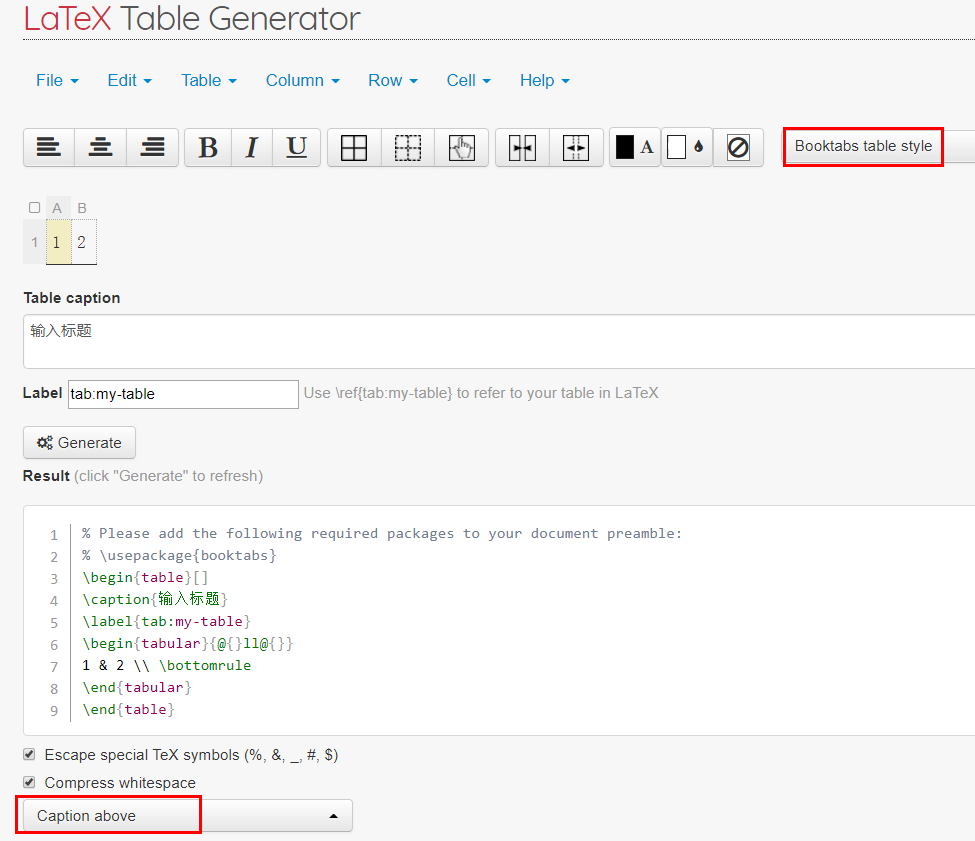
\includegraphics[width=1\textwidth]{HelperSection/figures/tableGenerator1.png}
 \caption{}
 \label{}
\end{figure}

制作的表格尽量为三线表,编辑好表格后,确保选择为Booktabs table style,然后Generate,复制黏贴就可以了。

\subsection{如何给表格添加脚注}
有时需要给表格添加脚注进行说明,例如:
\begin{table}[h]
\centering
\caption{表格标题}
\begin{threeparttable}
\label{表格引用标签}
\begin{tabular}{@{}ccccccc@{}}
\toprule
算法    & Minn  & Park  & Ren   & Fang  & Shao  & 改进算法\\ \midrule
时间($\mu s$) & 69.57 & 64.36 & 139.39 & 134.94 & 127.45 & 64.86    \\ \bottomrule
\end{tabular}
\begin{tablenotes}
        \footnotesize
        \item[] $N$是OFDM符号长度(不包括循环前缀),也即DFT点数  %此处加入注释信息
        \item[] $\theta$是滑动窗口起始抽样点%此处加入注释信息
      \end{tablenotes}
\end{threeparttable}
\end{table}

对应的代码为:
\begin{lstlisting}[language={tex}, caption={}]
\begin{table}[h] 
\centering
\caption{表格标题}
\begin{threeparttable} % 需要添加的部分
\label{表格引用标签}
\begin{tabular}{@{}ccccccc@{}}
\toprule
算法    & Minn  & Park  & Ren   & Fang  & Shao  & 改进算法\\ \midrule
时间($\mu s$) & 69.57 & 64.36 & 139.39 & 134.94 & 127.45 & 64.86    \\ \bottomrule
\end{tabular}

% 需要添加的部分
\begin{tablenotes}
        \footnotesize
        \item[] $N$是OFDM符号长度(不包括循环前缀),也即DFT点数  %此处加入注释*信息
        \item[] $\theta$是滑动窗口起始抽样点%此处加入注释**信息
      \end{tablenotes}
\end{threeparttable} % 需要添加的部分
\end{table}
\end{lstlisting}
\subsection{自查重模式下如何关闭表格显示}
在模板BIT-thesis-LaTex中(使用BIT-thesis-grd-jdh.cls格式控制文件)可以使用$\backslash$insertTable或者$\backslash$insertContents命令来实现。
\begin{lstlisting}[language={tex}, caption={}]
\insertTable{
	\begin{table}
		.......
	\end{table}
}
\insertContents{
	\begin{table}
		.......
	\end{table}
}
\end{lstlisting}
%%==================================================
%% abstract.tex for BIT Master Thesis
%% Edited by Jian dahao
%% version: 1.0
%% last update: May 10th, 2019
%%==================================================
\chapter{参考文献的使用}
\section{参考文献的管理}
论文模板使用BibTeX 处理参考文献,BibTeX 是最为流行的参考文献
数据组织格式之一。它的出现让我们摆脱手写参考文献条目的麻烦。当然,使用者也
可以手动编参考文献item,直接插入文档中。但是,有BibTeX 帮助,处理起参考文
献更为简单。我们还可以通过参考文献格式的支持,让同一份BibTeX 数据库生成不
同格式的参考文献列表。

参考文献的具体内容就是reference 文件夹下的references.bib,参考文献的元数据(名
称、作者、出处等) 以一定的格式保存在这些纯文本文件中。.bib 文件也可以理解为参
考文献的‘‘数据库’’,正文中所有引用的参考文件条目都会从这些文件中‘‘析出’’。控
制参考文献条目‘‘表现形式”(格式) 的是.bst 文件。.bst 文件定义了参考文献风格,使
用不同的参考文献风格能将同一个参考文献条目输出成不同的格式。当然,一个文档
只能使用一个参考文献风格。按照学校要求,本模板使用的是国标GBT7714 风格的
参考文献。
BibTeX 的工作过程是这样的:BibTeX 读取.aux(第一次运行latex 得到的) 查看参
考文献条目,然后到.bib 中找相关条目的信息,最后根据.bst 的格式要求将参考文献
条目格式化输出,写到.bbl 文件中。在运行latex 将.bbl 插入文档之前,可以用文本编辑器打开它,做一些小的修改。
\begin{lstlisting}[language={tex}, caption={.bib条目示例}]
@inproceedings{JianDahao2018,
author = {Jian, Dahao and Wu, Haixia and Gao, Wei and Jiang, Rongkun},
year = {2018},
month = {09},
pages = {1-5},
booktitle = {2018 IEEE International Conference on Signal Processing, Communications and Computing (ICSPCC)},
title = {A Novel Timing Synchronization Method Based on CAZAC Sequence for OFDM Systems},
doi = {10.1109/ICSPCC.2018.8567818}
}
\end{lstlisting}
.bib 数据库中的参考文献条目可以手动编写,也可以在google学术、百度学术等搜索中找到。注意要选择Bibtex格式。
\section{参考文献的编译}
bib文件与tex文件的编译时分开,需要用Bibtex先对bib文件进行编译,再编译tex。
\\
\fbox{\color{blue}如果无法正确显示参考文献,需要多编译几次。}

\section{参考文献的引用}
正文中引用参考文献时,用$\backslash$upcite\{key1,key2,key3...\} 可以产生“上标引用的参考文献”,如\upcite{JianDahao2018}。使用$\backslash$cite\{key1,key2,key3...\} 则可以产生水平引用的参考文献,例如\cite{JianDahao2018}。
如果要使用自查重模式时关闭引用标注的显示,在模板BIT-thesis-LaTex(使用BIT-thesis-grd-jdh.cls格式控制文件)中提供了$\backslash$nupcite和$\backslash$ncite可供使用(这两种命令在非自查重模式下,分别与$\backslash$upcite、$\backslash$cite等效)。

%%==================================================
%% abstract.tex for BIT Master Thesis
%% Edited by Jian dahao
%% version: 1.0
%% last update: May 10th, 2019
%%==================================================

\chapter{撰写论文中的注意事项}
\begin{enumerate}
\item{避免错别字}
\item{数学公式中的括号大小尽可能与公式高度保持一致,并且括号的使用严格按照\{[()]\}的顺序使用}
\item{图片的位置应该位于两个独立段落之间。}
\item{数值与单位之间应该具有空格,如1 dB。}
\item{公式定义处应该有冒号,例如定义公式如下\textbf{:}}
\item{公式引用时应该加上括号,例如:如公式(2.1)可知。}
\item{欢迎补充。。。。。。。。。}
\end{enumerate}




%(其后部分无编号)
\backmatter


\bibliography{references/references}
\end{document}
